\documentclass{article}
% translate with >> pdflatex -shell-escape <file>

% This file is an extract of the PGFPLOTS manual, copyright by Christian Feuersaenger.
% 
% Feel free to use it as long as you cite the pgfplots manual properly.
%
% See
%   http://pgfplots.sourceforge.net/pgfplots.pdf
% for the complete manual.
%
% Any required input files (for <plot table> or <plot file> or the table package) can be downloaded
% at
% http://www.ctan.org/tex-archive/graphics/pgf/contrib/pgfplots/doc/latex/
% and
% http://www.ctan.org/tex-archive/graphics/pgf/contrib/pgfplots/doc/latex/plotdata/

\usepackage{pgfplots}
\pgfplotsset{compat=newest}

\pagestyle{empty}

\begin{document}
\pgfplotsset{footnotesize,samples=10, domain=0:1,point meta min=0, point meta max=1}
\begin{center}% note that \centering uses less vspace...
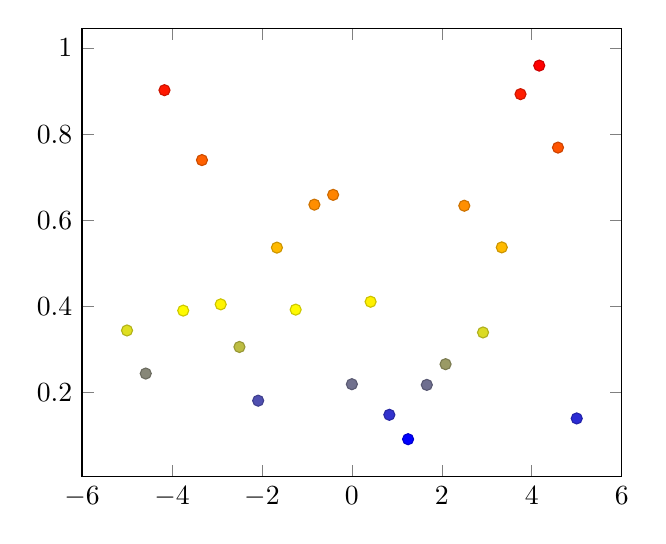
\begin{tikzpicture}
	\begin{axis}[colorbar,colorbar horizontal,colorbar to name={storedcolorbar}]
	\addplot[scatter,only marks,mark=*] {rnd};
	\end{axis}
\end{tikzpicture}
%
\begin{tikzpicture}
	\begin{axis}
	\addplot+[domain=0:1,mark=none,mesh] {x^2};
	\end{axis}
\end{tikzpicture}
%
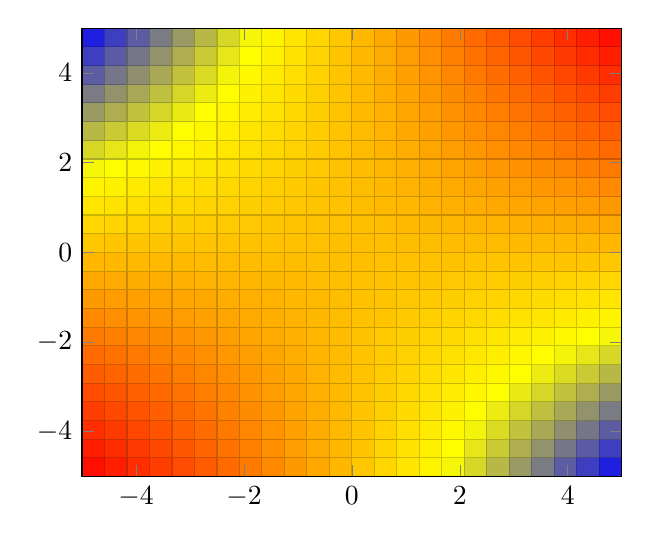
\begin{tikzpicture}
	\begin{axis}[view={0}{90}]
	\addplot3[surf] {x*y};
	\end{axis}
\end{tikzpicture}
\\

\ref{storedcolorbar}
\end{center}
\end{document}
